\documentclass[12pt,utf8,notheorems,compress]{beamer}

\usepackage[utf8]{inputenc}
\usepackage{default}

\usepackage{lmodern,listings}

% \usetheme{Berlin}
\usetheme{Warsaw}
%\useoutertheme{split}
\usecolortheme{seahorse}
\usepackage{kurier}
%\useinnertheme{rectangles}
\setbeamertemplate{navigation symbols}{}
\setbeamertemplate{footline}{}
\setbeamertemplate{headline}{}

\usepackage[english]{babel}
\usepackage[T1]{fontenc} % Trennung bei Woertern mit Umlauten
\usepackage{amssymb,amsmath,amsthm}
\usepackage{mathtools}
\usepackage{url,tikz}
\usepackage{graphicx}
\usepackage{comment,microtype}
\usepackage{listings}
\usepackage{pst-all}
\usepackage{xypic}

\graphicspath{{img/}}

\setlength\parskip{\medskipamount}
\setlength\parindent{0pt}

\title{Space Ops 101}

\subtitle{An Introduction to Spacecraft Control}

\author{Sven Prüfer}

\institute{German Space Operations Center}

\date{27.12.2018\\[0.5cm]
35c3}

%\titlegraphic{
%\includegraphics[width=6cm]{../images/Uni_Aug_Logo_IFM_RGB.png}
%}

\setlength{\unitlength}{1cm}

\begin{document}

\begin{frame}
 \titlepage
\end{frame}

\begin{frame}
  \frametitle{What we will not talk about ...}
  \begin{figure}[!ht]
    \centering
    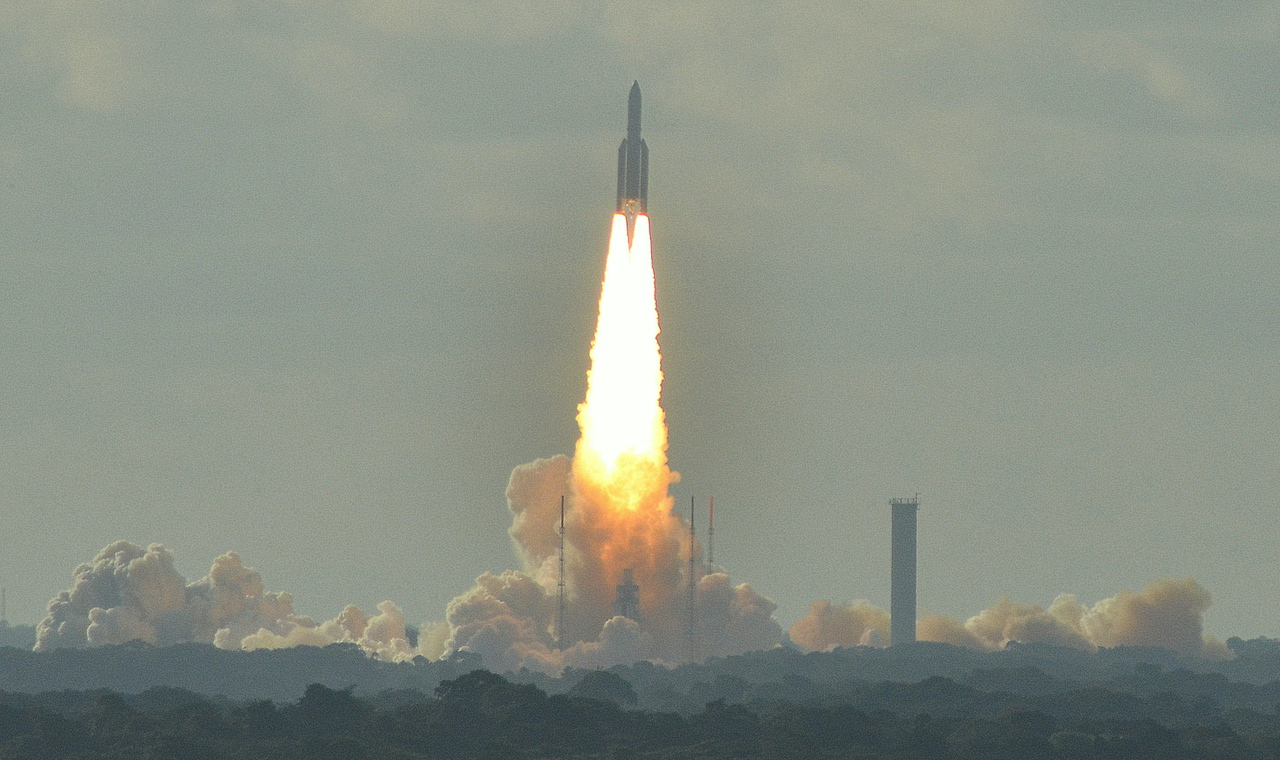
\includegraphics[width=\textwidth]{rocket-launch.jpg}
  \end{figure}
\end{frame}

\begin{frame}
  \frametitle{... but instead}
    \begin{figure}[!ht]
    \centering
    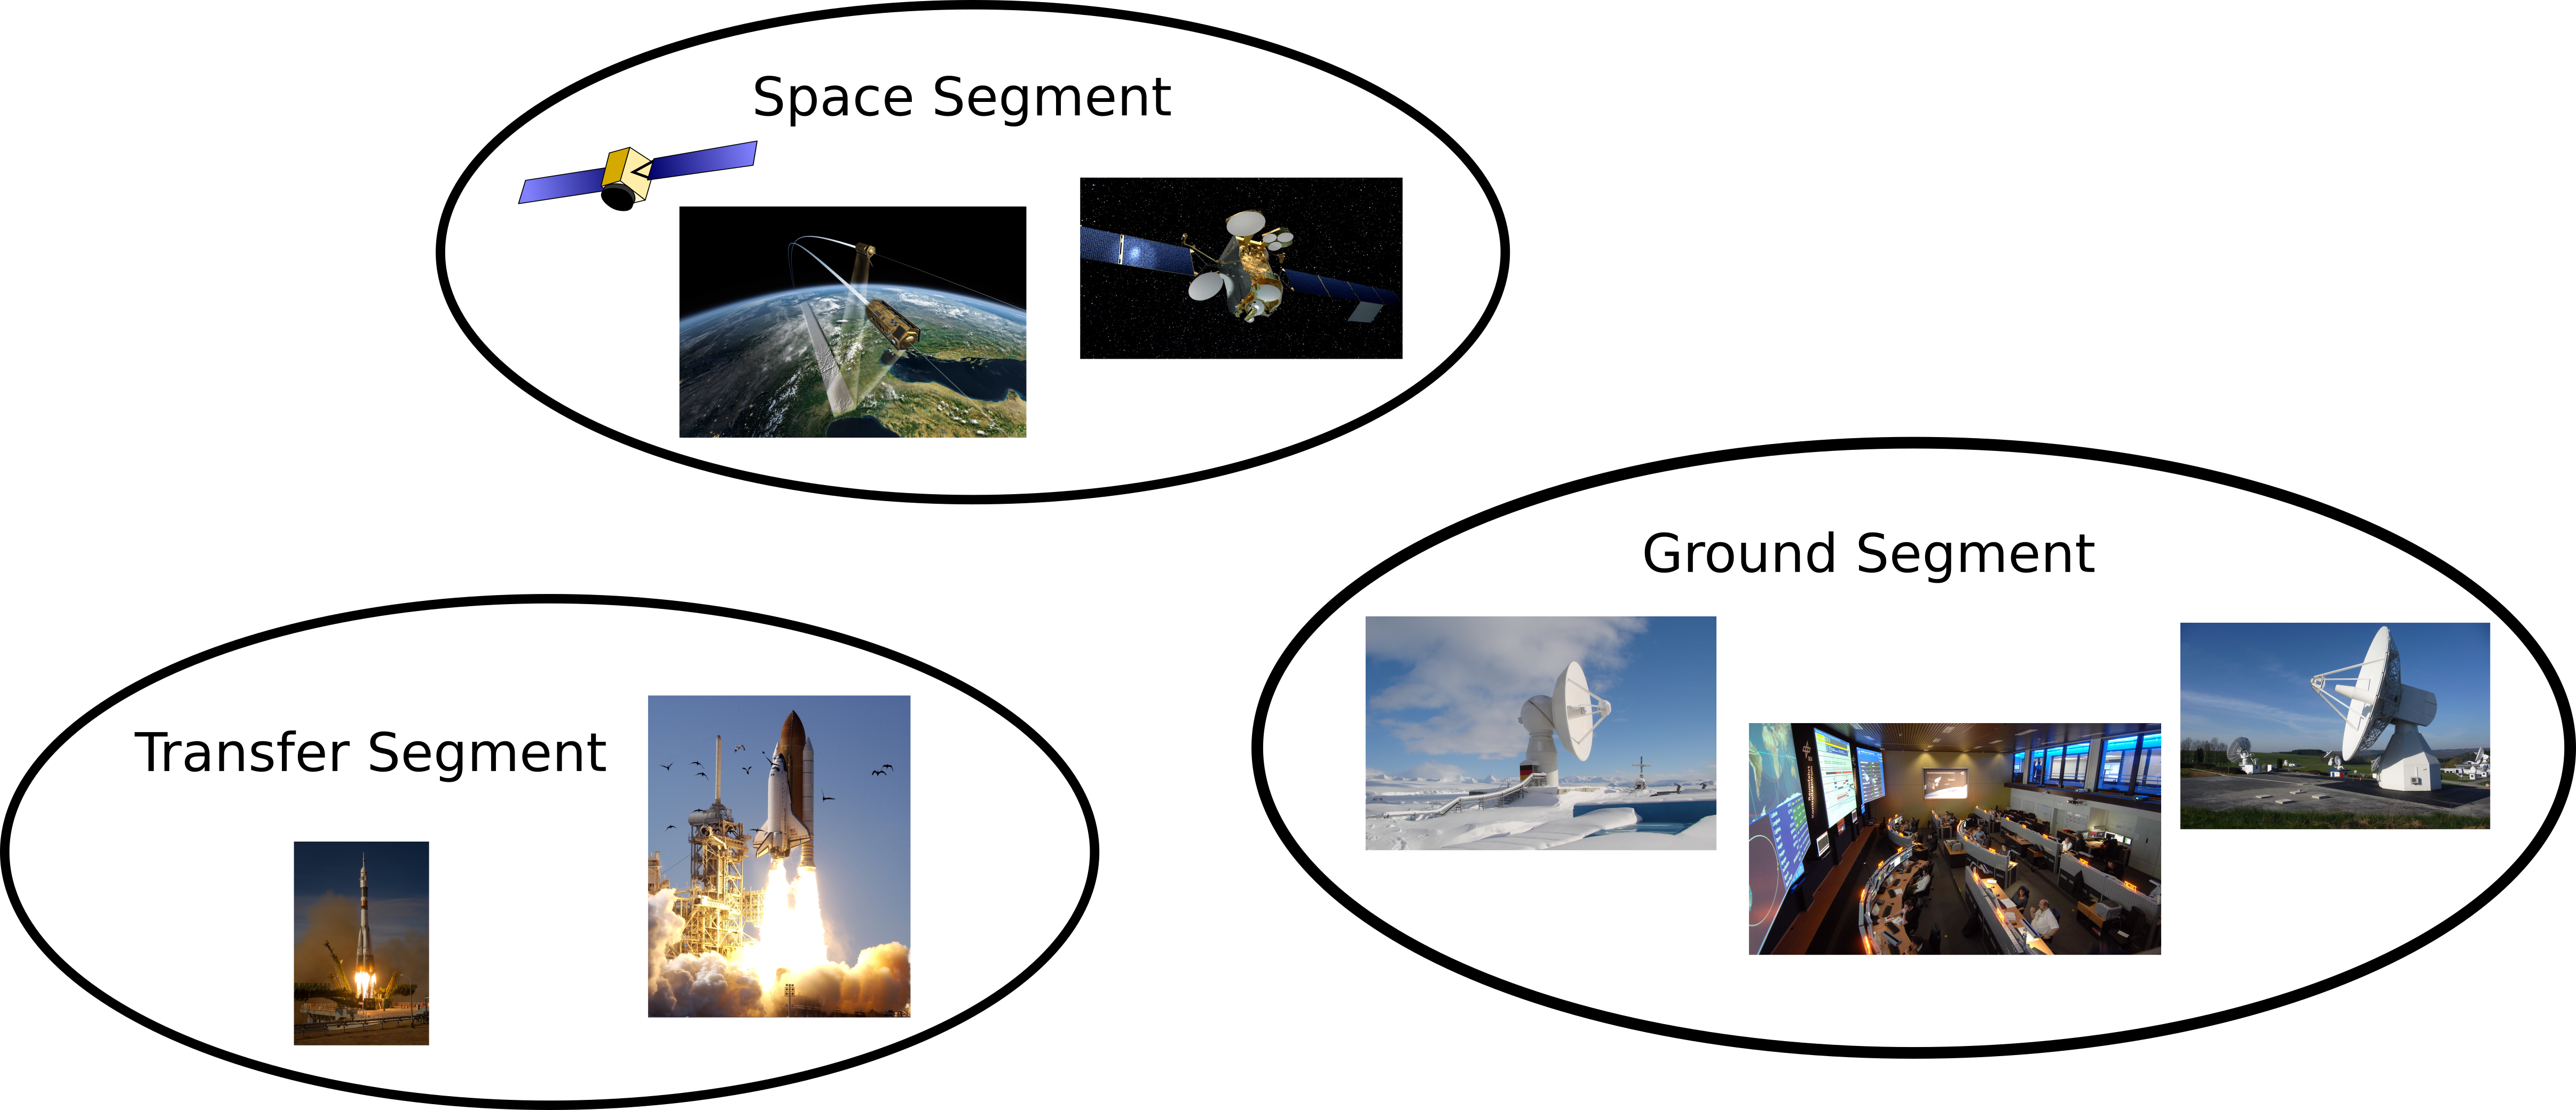
\includegraphics[width=1\textwidth]{segments.png}
  \end{figure}
\end{frame}

\begin{frame}
  \frametitle{... but instead}
    \begin{figure}[!ht]
    \centering
    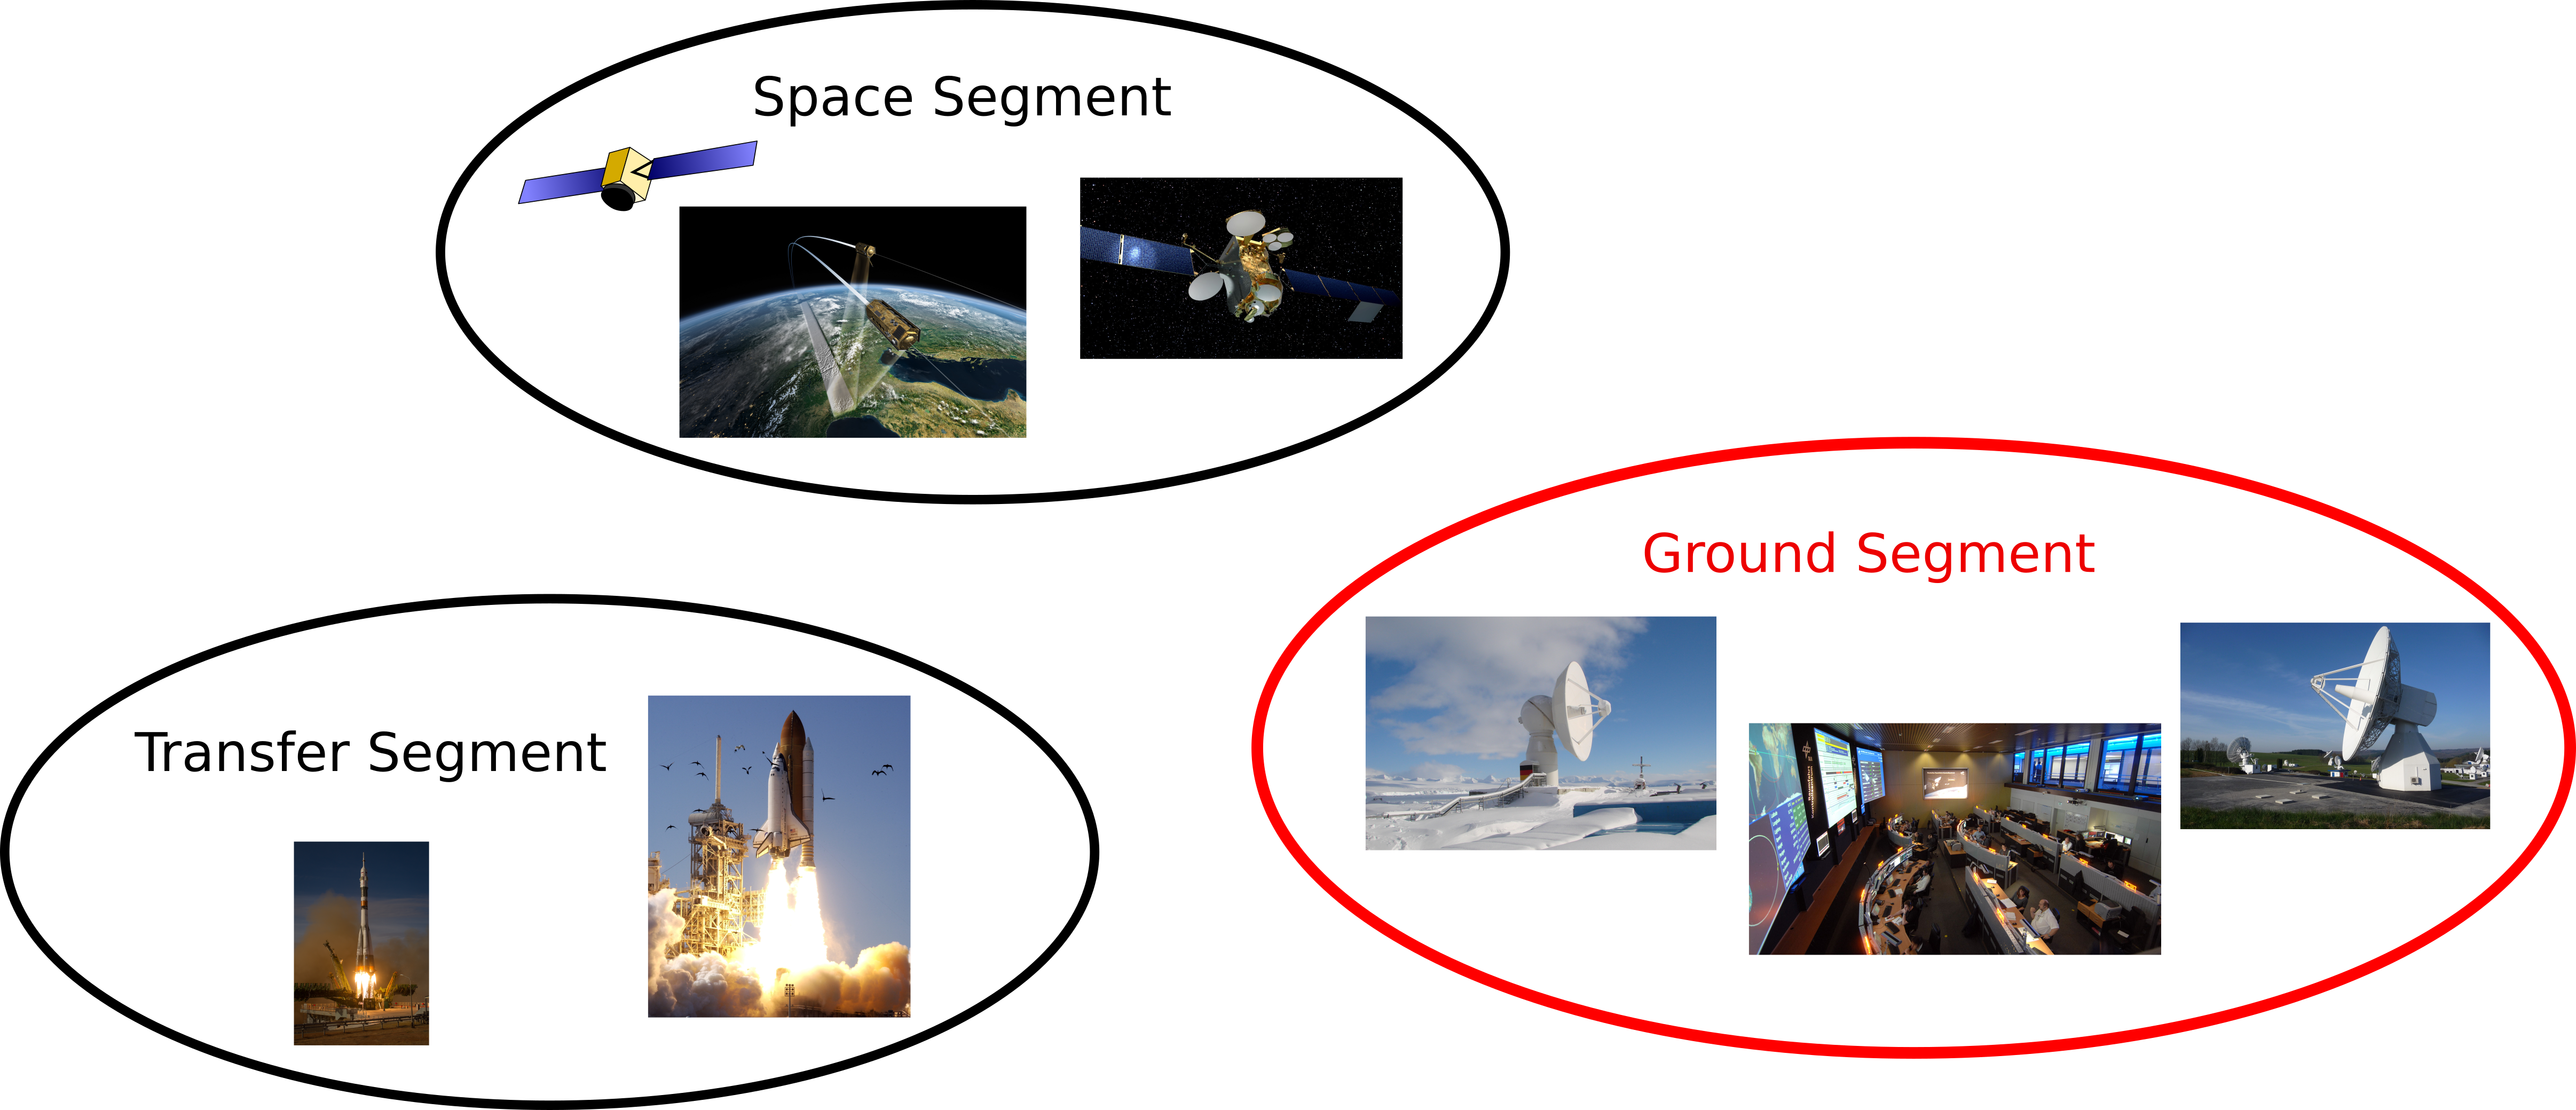
\includegraphics[width=1\textwidth]{segments-red.png}
  \end{figure}
\end{frame}

\begin{frame}
  \frametitle{Outline}
  \tableofcontents
\end{frame}

\begin{frame}
  \frametitle{What are we doing here?}
  \pause
  First, a mission needs a name ... such as
  \pause
  \begin{itemize}
    \item \textbf{G}ravity \textbf{R}ecovery \textbf{A}nd \textbf{C}limate \textbf{E}xperiment \pause or
    \item \textbf{Eu}glena and \textbf{C}ombined \textbf{R}egenerative \textbf{O}rganic-Food \textbf{P}roduction \textbf{i}n \textbf{S}pace.
  \end{itemize}
  \pause
  Next, we need a purpose:
  \pause
  \begin{itemize}
    \item Scientific? \pause
    \item Technology Demonstration? \pause
    \item Communications? \pause
    \item TV? \pause
    \item GNSS? \pause
    \item Espionage? \pause
    \item $\ldots$
  \end{itemize}
\end{frame}

\section{Basics of Spaceflight}

\subsection{Orbits}

\begin{frame}
  \frametitle{Why does a satellite not fall down?}
  \pause
  TODO add planet + satellite picture
\end{frame}

\begin{frame}
  \frametitle{LEO, MEO, GEO}
  \pause
  TODO add picture on distances
\end{frame}

\begin{frame}
  \frametitle{Some Statistics}
  \pause
  TODO add overview on number of satellites etc.
\end{frame}

\subsection{Communications}

\begin{frame}
  \frametitle{Pass}
  \pause
  TODO add picture showing pass
\end{frame}

\begin{frame}
  \frametitle{Link Budget}
  \pause
  TODO add picture link budget
\end{frame}

\begin{frame}
  \frametitle{Frequency Range}
  \pause
  TODO add picture absorption in athmosphere
\end{frame}

\begin{frame}
  \frametitle{Up- and Downlink}
  \pause
  TODO explain purpose of up- and downlinks
\end{frame}

\subsection{Phases of Mission Operations}

\begin{frame}
  \frametitle{LEOP}
  \pause
  TODO explain purpose of LEOP
\end{frame}

\begin{frame}
  \frametitle{Commisioning or IOT}
  \pause
  TODO explain purpose of IOT
\end{frame}

\begin{frame}
  \frametitle{Routine}
  \pause
  TODO explain purpose of Routine (mention monitoring + machine learning)
\end{frame}

\begin{frame}
  \frametitle{EOL}
  \pause
  TODO explain EOL
\end{frame}

\section{Procedures}

\subsection{TC, TTC and Telemetry}

\begin{frame}
  \frametitle{TCs and TTCs}
  \pause
  TODO explain TCs and TTCs
\end{frame}

\begin{frame}
  \frametitle{Examples for TTCs}
  \pause
  TODO example TTC
\end{frame}

\begin{frame}
  \frametitle{Telemetry}
  \pause
  TODO example TTC
\end{frame}

\subsection{Flight Procedures}

\begin{frame}
  \frametitle{Purpose of Flight Procedures}
  \pause
  TODO explain purpose of flight procedures
\end{frame}

\begin{frame}
  \frametitle{Example of a Flight Procedure}
  \pause
  TODO picture of a flight procedure
\end{frame}

\subsection{Ground Procedures}

\begin{frame}
  \frametitle{Example of a Ground Procedure}
  \pause
  TODO picture of a ground procedure
\end{frame}

\section{Subsystems}

\begin{frame}
  \frametitle{FDS and AOCS}
  \pause
  TODO explain purpose FDS and AOCS, mention Fortran
\end{frame}

\begin{frame}
  \frametitle{Safe Modes}
  \pause
  TODO add picture for various modes
\end{frame}

\begin{frame}
  \frametitle{Data and TM/TC}
  \pause
  TODO explain purpose Data and TM/TC
\end{frame}

\begin{frame}
  \frametitle{SCOS}
  \pause
  TODO add picture SCOS
\end{frame}

\begin{frame}
  \frametitle{PTR}
  \pause
  TODO explain PTR, show heat curve, mention MLI
\end{frame}

\begin{frame}
  \frametitle{MIPL}
  \pause
  TODO explain purpose
\end{frame}

\begin{frame}
  \frametitle{SoE}
  \pause
  TODO add picture sample SoE
\end{frame}

\section{Contingencies}

\begin{frame}
  \frametitle{Flight and Engineering Model}
  \pause
  TODO explain purpose of engineering model
\end{frame}

\begin{frame}
  \frametitle{Procedure in Case of Contingency}
  \pause
  TODO add picture contingency procedure
\end{frame}

\begin{frame}
  \frametitle{Example Contingency: TvSat-1}
  \pause
  TODO add picture and explanation TcSat-1
\end{frame}





% \begin{frame}
%   \frametitle{Example}
%   \begin{figure}[!ht]
%     \centering
%     \def\svgwidth{0.8\textwidth}
%     \input{../images/example-hurwitz-cover.pdf_tex}
%   \end{figure}
% \end{frame}


\begin{frame}
  \frametitle{Questions?}
  \vfill
  \begin{center}
    \Large Thank you and enjoy the rest of the congress!
  \end{center}
  \vfill
\end{frame}


\end{document}
